\subsubsection{UC5 - Login Manuale}
\begin{figure}[h]
	\centering
	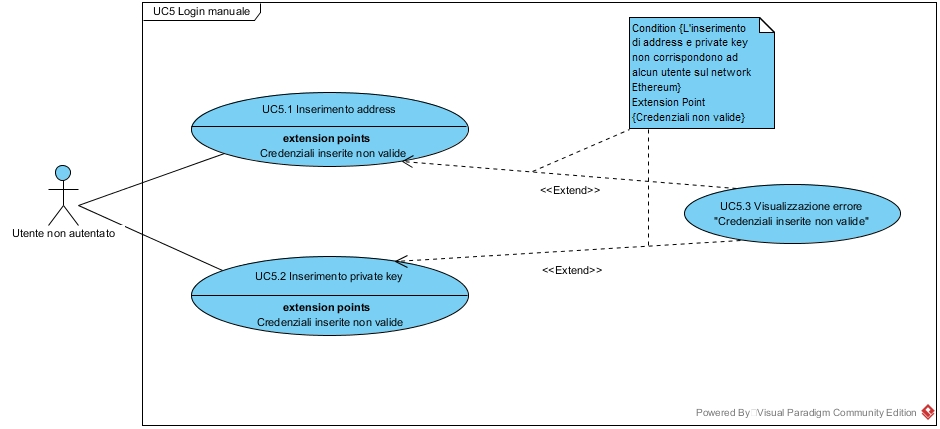
\includegraphics[width=\linewidth]{res/img/UC5.jpg}
	\caption{Diagramma UC5 - Login manuale}
\end{figure}
\begin{itemize}
	\item \textbf{Attori primari:} Utente non autenticato;
	\item \textbf{Attori secondari:} \textit{Ethereum\glo} Network;
	\item \textbf{Descrizione:} l'utente, mediante il comando "login" ha la possibilità di autenticarsi al network \textit{Ethereum\glo} inserendo manualmente da \textit{CLI\glo} il proprio address e \textit{private key\glos} e, contestualmente, salvare in automatico le credenziali di accesso su un file sul proprio dispositivo; 
	\item \textbf{Pre-condizioni:} l'utente ha visualizzato la guida introduttiva e desidera autenticarsi manualmente;
	\item \textbf{Post-condizioni:} il sistema avrà autenticato o meno l'utente a seconda dei valori di accesso inseriti dalla \textit{CLI\glos};
	\item \textbf{Scenario principale:} 
	\begin{enumerate}
		\item L'utente scriverà un comando da \textit{CLI\glos}, composto nel seguente modo:
		\begin{itemize}
			\item nome del comando "login";
			\item address;
			\item \textit{private key\glos}.
		\end{itemize} 
		\item Verrà visualizzato a schermo un messaggio relativo all'esito dell'autenticazione.
	\end{enumerate}	
	\item \textbf{Inclusioni:}
		\begin{itemize}
		\item\textbf{UC3}: ogni qualvolta viene eseguito il login manuale da parte dell'utente, viene salvato sul dispositivo un file contenente le credenziali.
	\end{itemize}  
\end{itemize}
